%%%Preamble
\documentclass[12pt]{article}
\usepackage{epsfig, amsfonts, cite, amssymb}
\usepackage{subfigure}
\usepackage{array}
\usepackage{float}
\usepackage{enumitem}
\usepackage{indentfirst}
\usepackage{boldline}
\usepackage[usenames,dvipsnames,svgnames,table]{xcolor}
\usepackage{amsmath}

%%% Use these when running Text Verifications
%\usepackage[T1]{fontenc}        
%\usepackage[utf8]{inputenc}     
%\usepackage[adobe-utopia]{mathdesign}
%\usepackage{printlen}

\voffset=0in \hoffset=0in \textwidth=6.3in \textheight=8.3in
\setlength{\oddsidemargin}{0in} \setlength{\textwidth}{6 in}
\thispagestyle{empty}

\begin{document}

\begin{figure*}[htb]
\subfigure{
\includegraphics[width=2.5in]{wne.eps} }
\hfil \hspace{.5in}
\subfigure{
\includegraphics[width=2.5in]{department.eps} }
\end{figure*}

%%%Header
\begin{center}
{\Large {\bf CPE 462/562 VHDL: Simulation \& Synthesis}}\\
\vspace{0.2in}
{\Large{Project 3: Digital Alarm Clock Design and Implementation}} \\
\vspace{0.2in}

%%%Cover Page
Katelyn Charbonneau\\
Email: kc325844@wne.edu\\
Date: 11/20/2017\\
\end{center}

%%%Text Verifications
%This text is \fontname\font\ with font size \csname f@size\endcsname{}
%and \verb|\baselineskip| =~\the\baselineskip =~\uselengthunit{mm}\printlength{\baselineskip}.

%%% END of Cover Page
\newpage

\section{Objective} \label{sec:obj}
The objectives of the project are to design an implement a configurable digital alarm clock; be able to write VHDL code to design said clock using a wide variety of coding techniques; and implement the clock on the Altera DE-115 FPGA.

\section{Design Procedure} \label{sec:desproc}
The top level design block is shown in Figure \ref{fig:toplevel}.

\begin{figure}[!h]
\setlength{\belowcaptionskip}{-10pt}
\begin{center}
\includegraphics[scale=0.6]{alarm_clock_top_level.png}
\caption{Alarm Clock Top Level Block}
\label{fig:toplevel}
\end{center}
\end{figure}

Where Alarm, Clock, Hour, and Minute Set are push buttons, Alarm Enable and Reset are switches, Alarm and AM/PM are LEDs, and the Hex Displays are 6 vectors; one for each seven segment display used in this project.

\vspace{14.5pt}

The digital clock supports setting the time and alarm time on a 12-hour clock with an asynchronous reset.  When the current clock time is equal to the alarm time, the alarm will signal and can be turned off with the Alarm Enable switch.\par
The push buttons on the FPGA are not debounced well.  As such, a custom debounce routine was written for each of the buttons; this was then included as a component in the main design.  The process used in this code is shown on the next page in Figure \ref{fig:debounce}.

\newpage

\begin{figure}[H]
\setlength{\belowcaptionskip}{-10pt}
\begin{center}
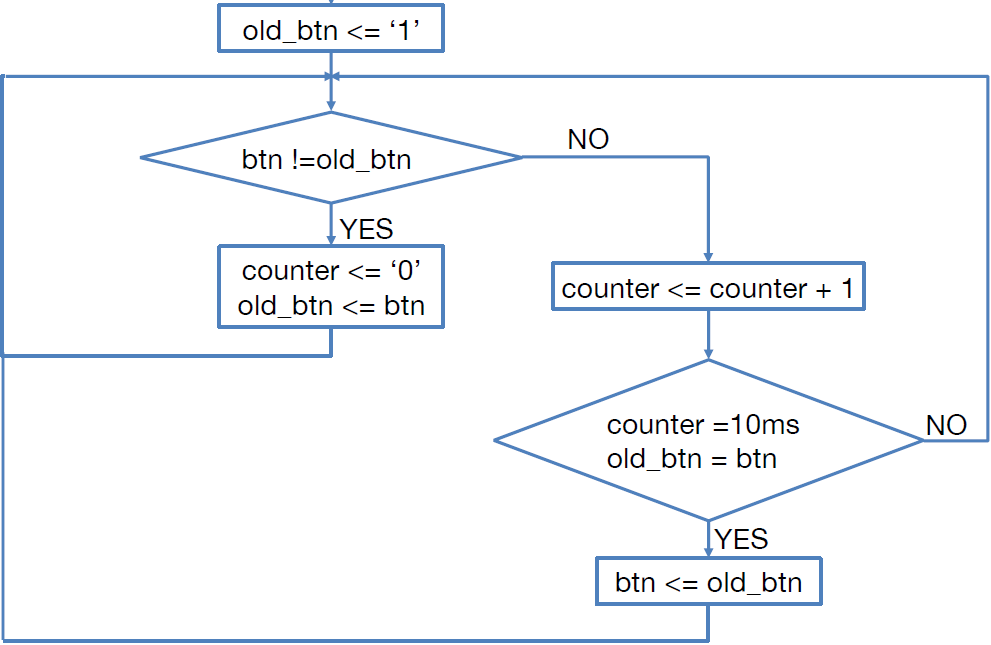
\includegraphics[scale=0.5]{debounce_algorithm.png}
\caption{The debouncing flow chart}
\label{fig:debounce}
\end{center}
\end{figure}

Because the clock needs to increment every second, we need a 1Hz clock to drive it.  Since the FPGA's clock is 50MHz, a new 1Hz clock was made by "slowing down" the original.  This was done by counting how many rising edges of the original clock are needed for a second to pass, and changing the value of the 1Hz clock when that many edges passed.  The clock counts time by incrementing the one's place of the seconds value by 1 each second, which then cascades down.  For example, a 9 in the one's place would next revert to 0 and increase the ten's place by 1; a 5 in the ten's place would next revert to 0 and increase the one's place of minutes, and so on.  The hours reset from "12" back to "01", and the AM/PM signal changes when hours advance from "11" to "12".  Hitting the reset switch sets both the clock time and alarm time to 12:00:00 midnight and locks them both at that value until reset is released.\par
When the clock and alarm times are equal, the alarm signal is set to high and will remain high for a minute.  During this minute, it can be turned off by flipping the alarm switch, and will automatically turn itself off after a minute has passed.

\newpage

\section{Simulation Results} \label{simresults}

\begin{figure}[H]
\begin{center}
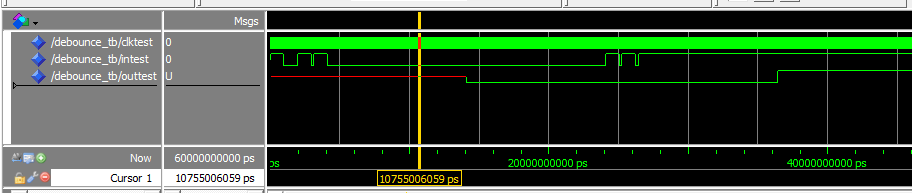
\includegraphics[scale=0.6]{debounce_sim.png}
\caption{Showing debouncing program works with simulated bouncy input}
\label{fig:simdb}
\end{center}
\end{figure}

\newpage

\section{Demonstration on FPGA} \label{demo}
The design was synthesized onto the Altera Cyclone IV E DE2-115F29C7 FPGA.
\begin{itemize}
\item User Controls:
	\begin{itemize}
	\item Alarm Set: Key 3
	\item Clock Set: Key 2
	\item Hour Set: Key 1
	\item Minute Set: Key 0
	\item Alarm Enable: Switch 0
	\item Reset: Switch 1
	\end{itemize}
\item Output Displays:
	\begin{itemize}
	\item Hours: Hex 7 and 6
	\item Minutes: Hex 5 and 4
	\item Seconds: Hex 3 and 2
	\item Alarm: Red LED 0 (LEDR0)
	\item AM/PM Indicator: Green LED 8 (LEDG8)
	\end{itemize}
\end{itemize}

\begin{figure}[H]
\begin{center}
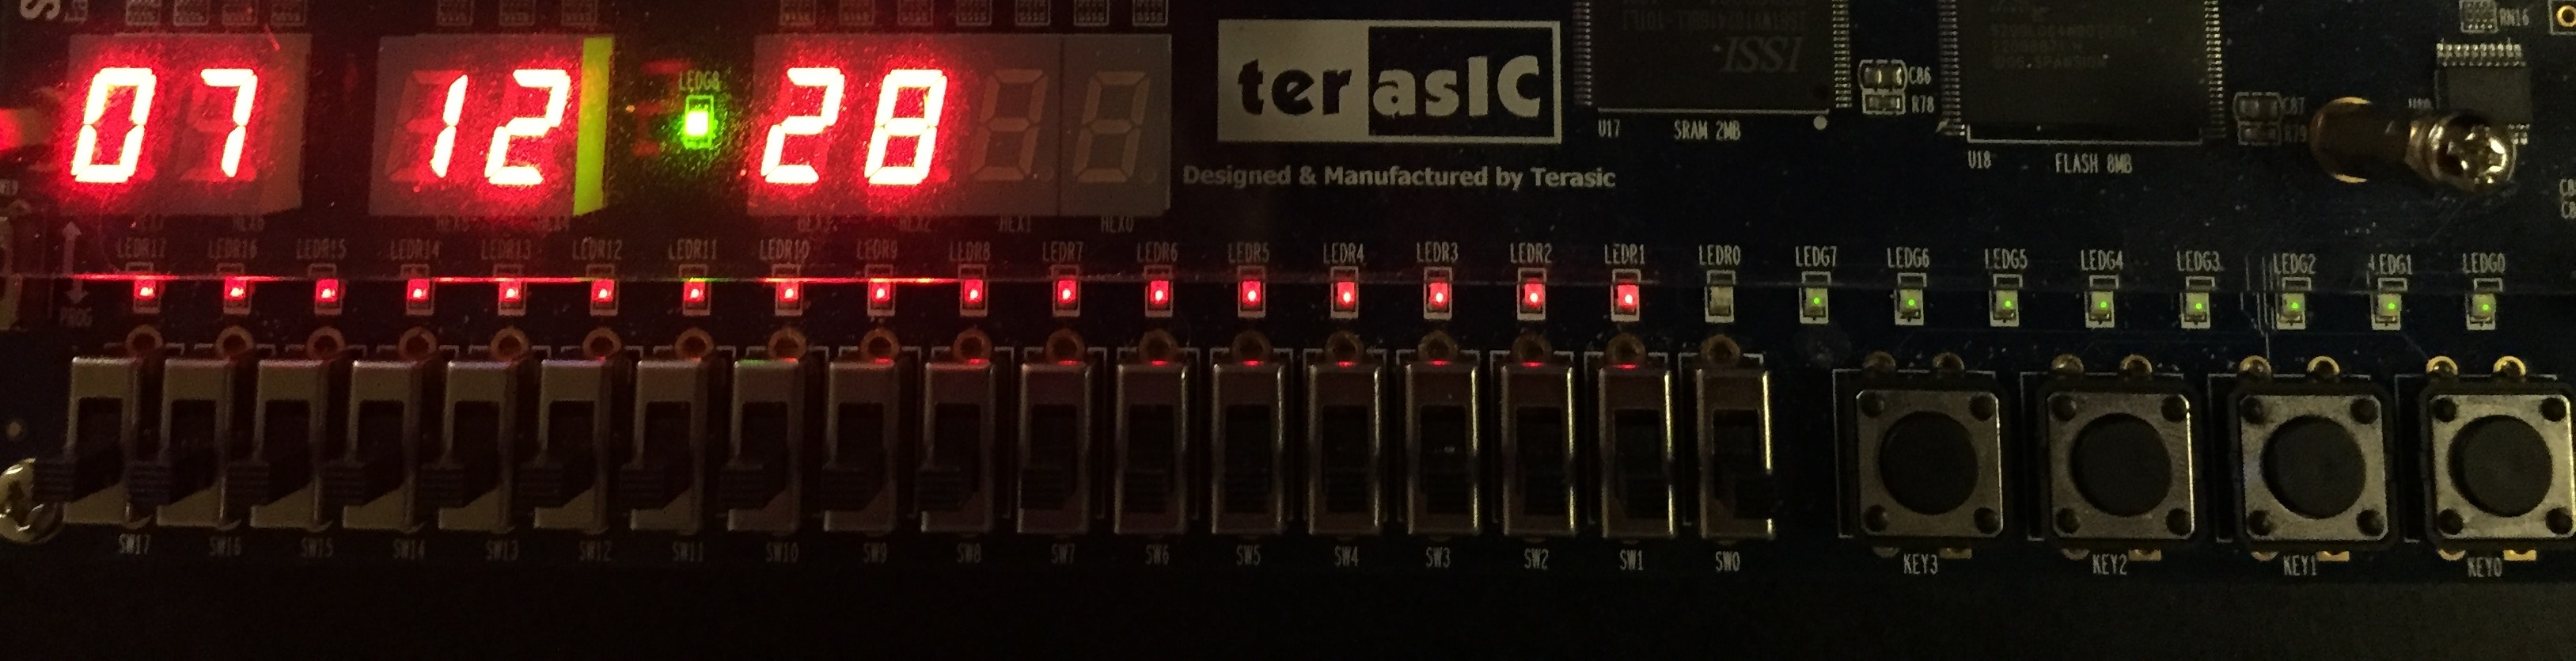
\includegraphics[scale=0.1]{board_1.png}
\caption{Displaying clock time}
\label{fig:board1}
\end{center}
\end{figure}

\begin{figure}[H]
\begin{center}
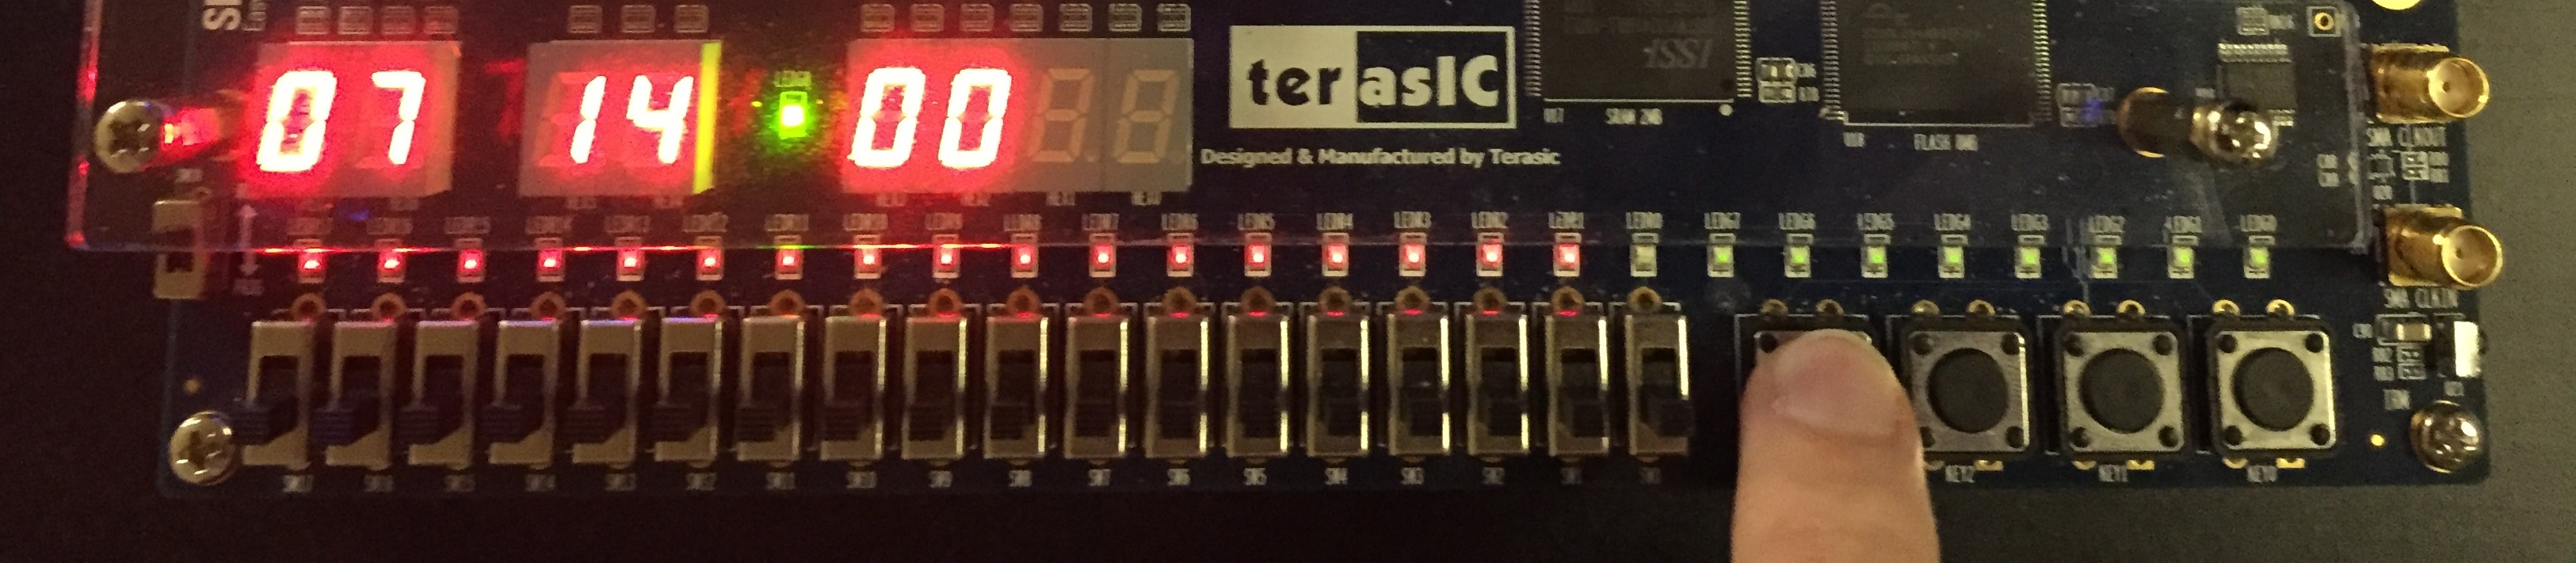
\includegraphics[scale=0.1]{board_2.png}
\caption{Displaying alarm time}
\label{fig:board2}
\end{center}
\end{figure}

\begin{figure}[H]
\begin{center}
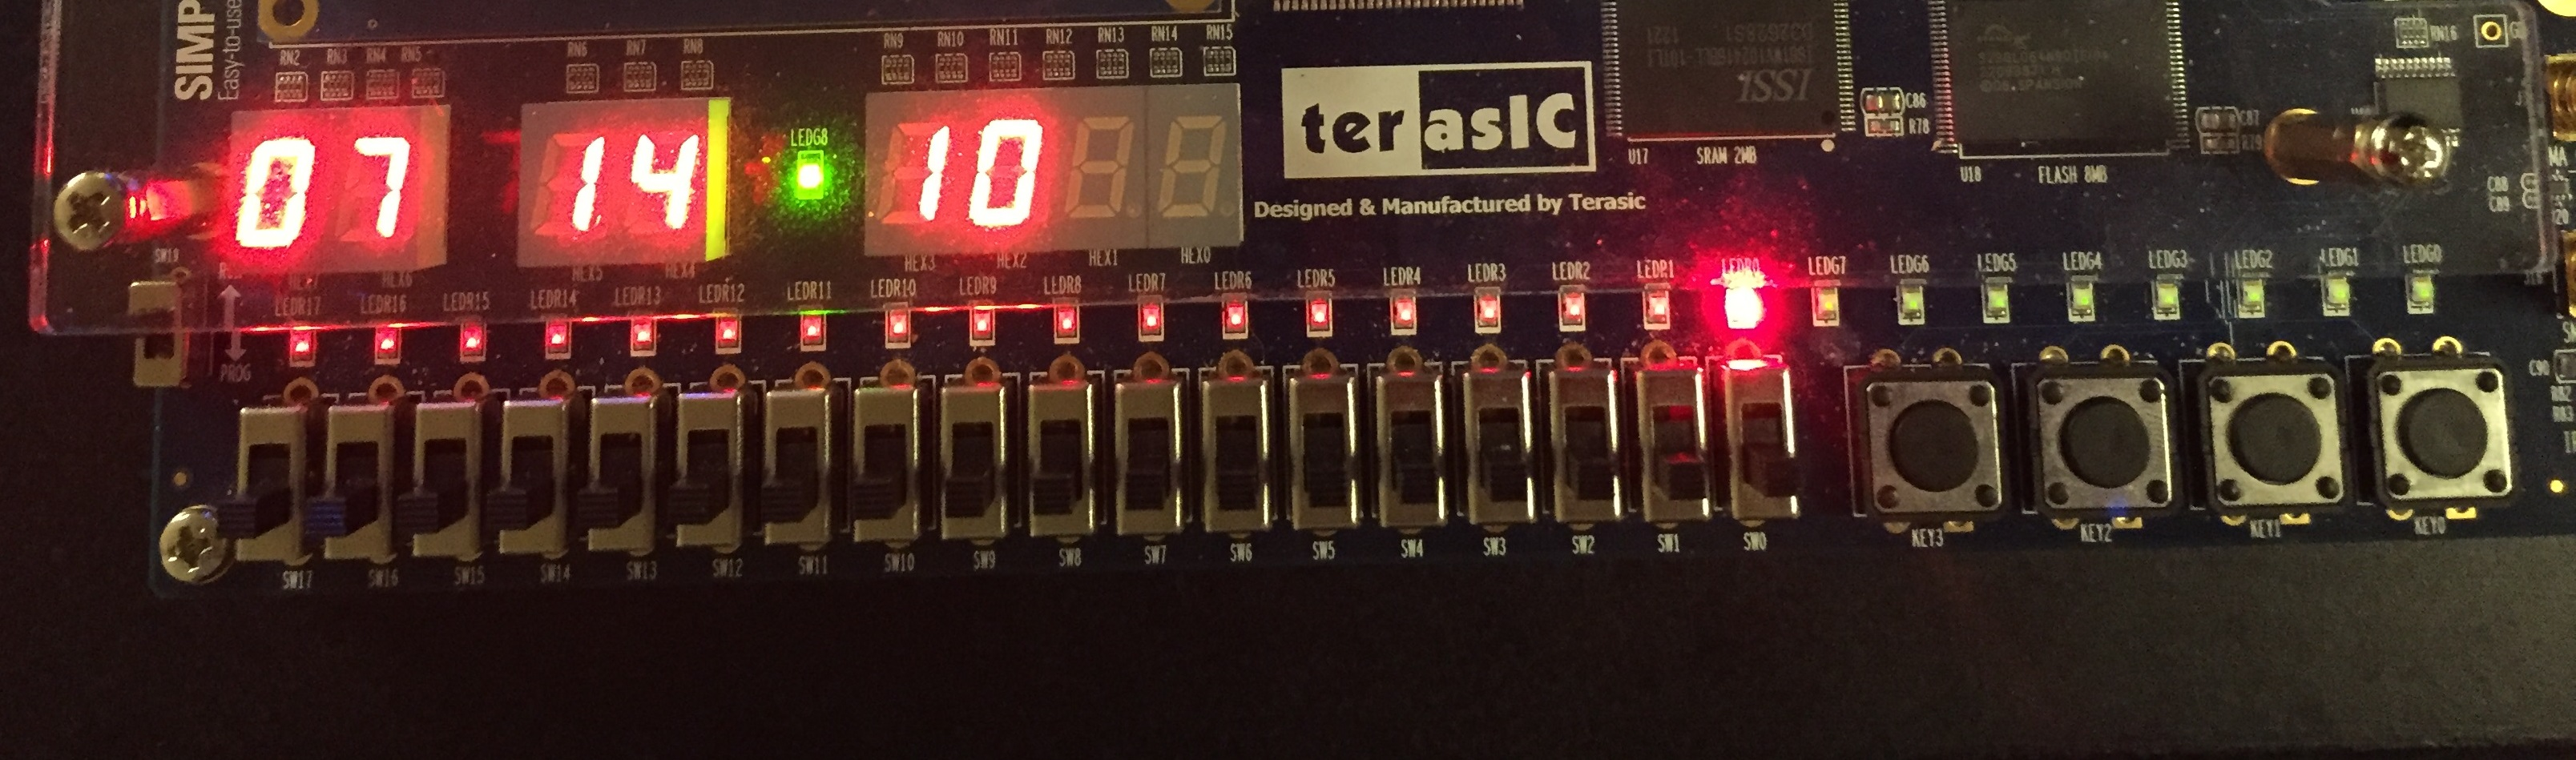
\includegraphics[scale=0.1]{board_3.png}
\caption{Alarm is set high}
\label{fig:board3}
\end{center}
\end{figure}

\begin{figure}[H]
\begin{center}
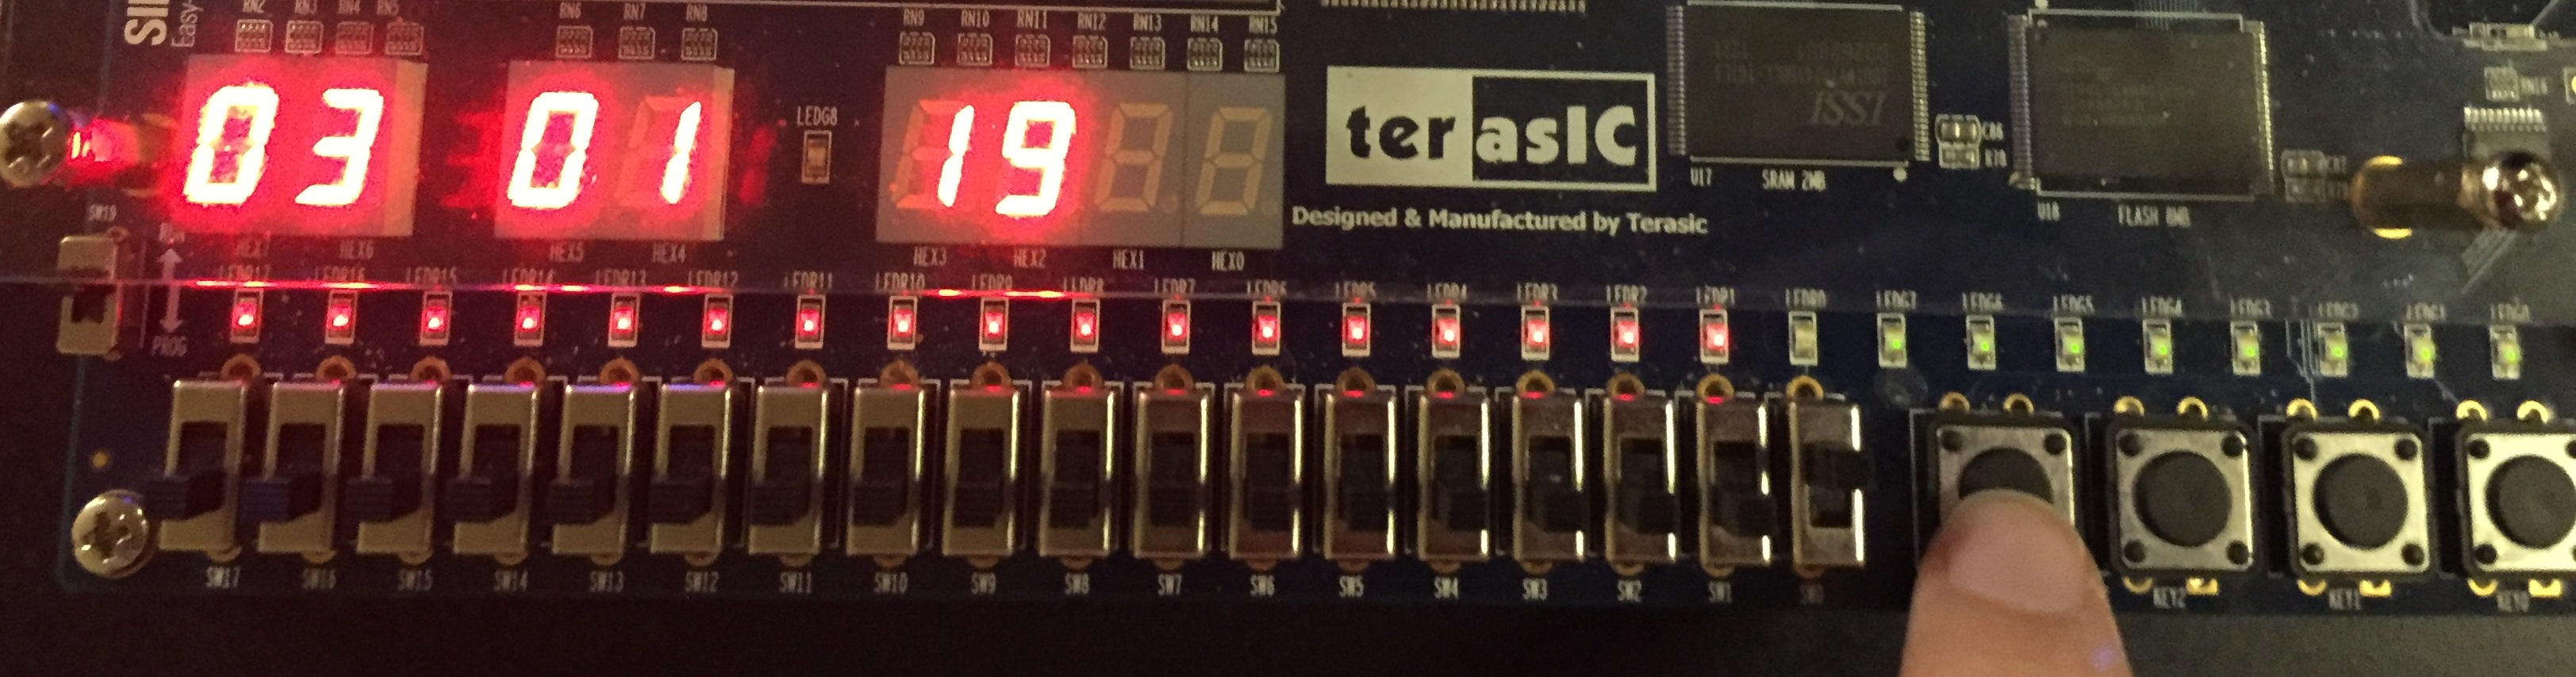
\includegraphics[scale=0.1]{board_4.png}
\caption{Alarm is set high, but the switch is set to turn it off}
\label{fig:board4}
\end{center}
\end{figure}

\begin{figure}[H]
\begin{center}
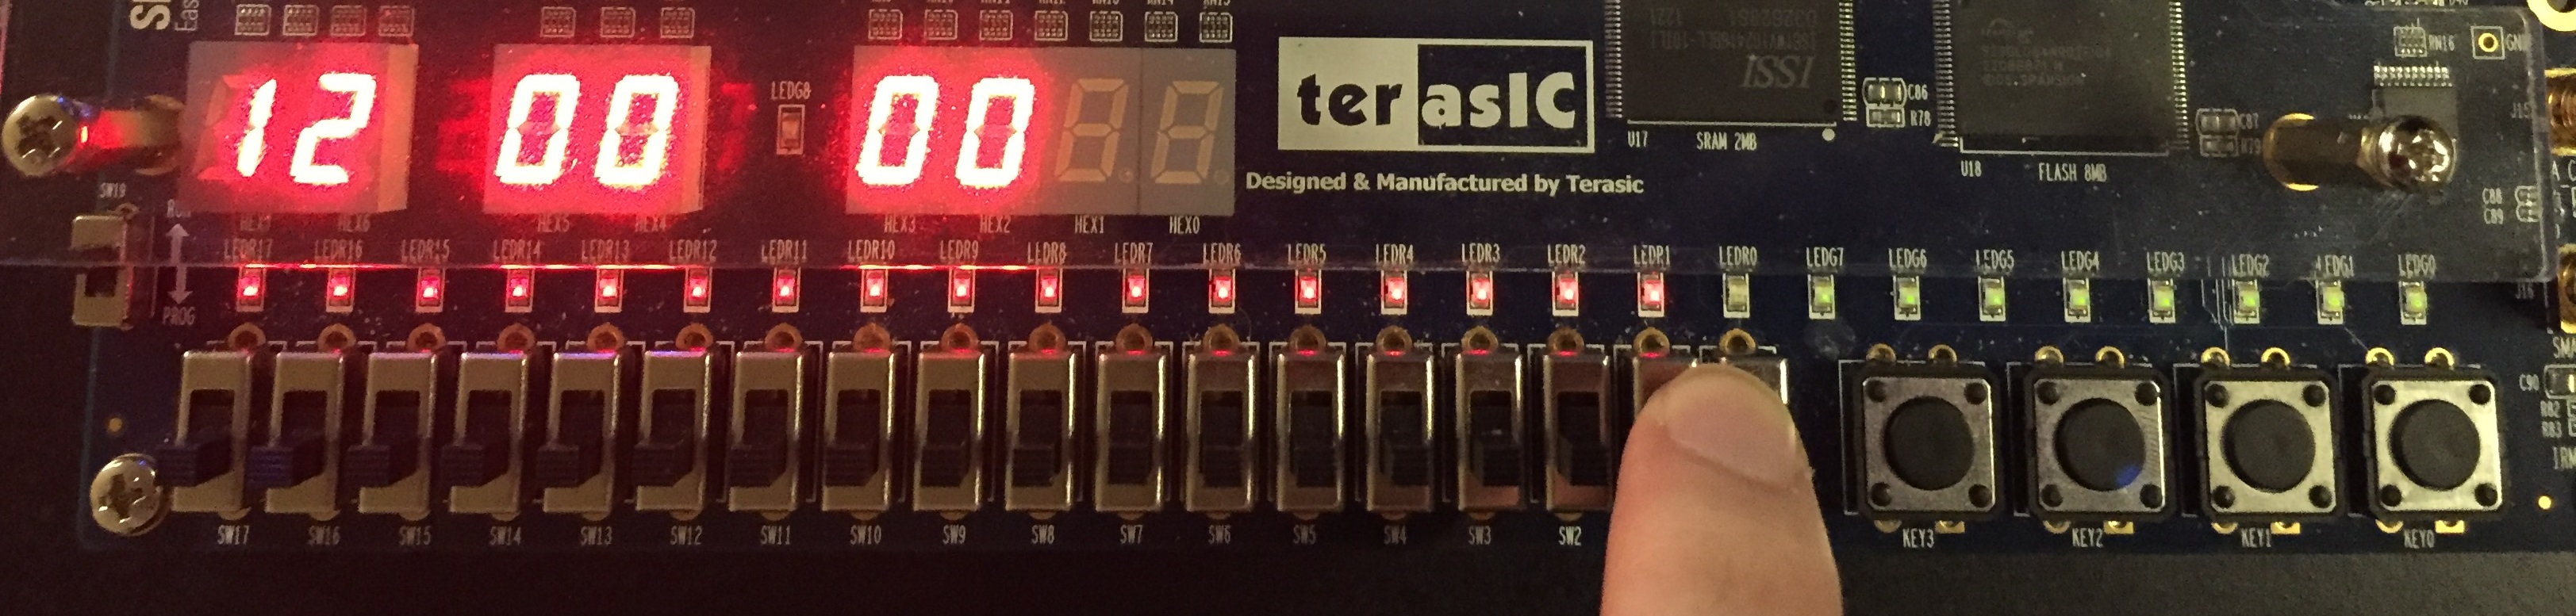
\includegraphics[scale=0.1]{board_5.png}
\caption{Reset is set}
\label{fig:board5}
\end{center}
\end{figure}

\newpage

\section{Conlusion} \label{cncl}
The project simulated and synthesized correctly.  The code required sufficient knowledge of structural, concurrent, and sequential VHDL. A package was designed to compartmentalize the code to make it easier to read and debug.  Recently learned functions and procedures were used within this package, as well as the declaration of the debounce component to make the main code cleaner.  Some improvements need to made.  One of these is the way the alarm status/enable switch functions - it could operate in a much more user-friendly manner.  Also, the clock pauses while the user is changing the time (not the alarm time).  Again, this could be a user-friendly improvement to make to the code to either allow the clock to continue ticking while the Clock Set key is pressed, or force the seconds to "00" while this is happening so the clock will always be set to an even minute.

\end{document} 
